% Hlavicka pro protokoly z fyzikalniho praktika.
% Verze pro: LaTeX
% Verze hlavicky: 22. 2. 2007
% Autor: Ustav fyziky kondenzovanych latek
% Ke stazeni: www.physics.muni.cz/ufkl/Vyuka/
% Licence: volne k pouziti, nejlepe k vcasnemu odevzdani protokolu z Vaseho mereni.

\documentclass[a4paper,11pt]{article}

% Kodovani (cestiny) v dokumentu: utf-8
%\usepackage[cp1250]{inputenc}	% Omezena stredoevropska kodova stranka, pouze MSW.
\usepackage[utf8]{inputenc}	% Doporucujeme pouzivat UTF-8 (unicode).
\usepackage[T1]{fontenc}
\usepackage{lmodern}

%%% Nemente:
\usepackage[margin=2cm]{geometry}
\newtoks\jmenopraktika \newtoks\jmeno \newtoks\datum
\newtoks\obor \newtoks\skupina \newtoks\rocnik \newtoks\semestr
\newtoks\cisloulohy \newtoks\jmenoulohy
\newtoks\tlak \newtoks\teplota \newtoks\vlhkost
\usepackage{amsmath}
\usepackage{mathtools}
\usepackage{graphicx}
\usepackage{multirow}

\usepackage{pgfplotstable} 
\usepackage{booktabs}

\graphicspath{ {./images/} }
%%% Nemente - konec.


%%%%%%%%%%% Doplnte pozadovane polozky:

\jmenopraktika={Fyzikální praktikum 3}  % nahradte jmenem vaseho predmetu
\jmeno={Artem Gorodilov}            % nahradte jmenem mericiho
\datum={15. ~dubna  2024}        % nahradte datem mereni ulohy
\obor={Astrofyzika}                     % nahradte zkratkou vami studovaneho oboru
\skupina={Po 14:00}            % nahradte dobou vyuky vasi seminarni skupiny
\rocnik={II}                  % nahradte rocnikem, ve kterem studujete
\semestr={II}                 % nahradte semestrem, ve kterem studujete

\cisloulohy={I}               % nahradte cislem merene ulohy
\jmenoulohy={Rutherfordův experiment} % nahradte jmenem merene ulohy

\tlak={979}                   % nahradte tlakem pri mereni (v hPa)
\teplota={21.4}               % nahradte teplotou pri mereni (ve stupnich Celsia)
\vlhkost={46}               % nahradte vlhkosti vzduchu pri mereni (v %)

%%%%%%%%%%% Konec pozadovanych polozek.


%%%%%%%%%%% Uzitecne balicky:
\usepackage[czech]{babel}
\usepackage{graphicx}
\usepackage{amsmath}
\usepackage{xspace}
\usepackage{url}
\usepackage{indentfirst}
\usepackage{listings}
\usepackage{subcaption}
\usepackage{caption}
\usepackage{tabularx}
\usepackage[labelformat=parens,labelsep=quad,skip=3pt]{caption}

%%%%%% Zamezeni parchantu:
\widowpenalty 10000 \clubpenalty 10000 \displaywidowpenalty 10000
%%%%%% Parametry pro moznost vsazeni vetsiho poctu obrazku na stranku
\setcounter{topnumber}{3}	  % max. pocet floatu nahore (specifikace t)
\setcounter{bottomnumber}{3}	  % max. pocet floatu dole (specifikace b)
\setcounter{totalnumber}{6}	  % max. pocet floatu na strance celkem
\renewcommand\topfraction{0.9}	  % max podil stranky pro floaty nahore
\renewcommand\bottomfraction{0.9} % max podil stranky pro floaty dole
\renewcommand\textfraction{0.1}	  % min podil stranky, ktery musi obsahovat text
\intextsep=8mm \textfloatsep=8mm  %\intextsep pro ulozeni [h] floatu a \textfloatsep pro [b] or [t]

% Tecky za cisly sekci:
\renewcommand{\thesection}{\arabic{section}.}
\renewcommand{\thesubsection}{\thesection\arabic{subsection}.}
% Jednopismenna mezera mezi cislem a nazvem kapitoly:
\makeatletter \def\@seccntformat#1{\csname the#1\endcsname\hspace{1ex}} \makeatother

\begin{document}

\thispagestyle{empty}

{
\begin{center}
\sf 
{\Large Ústav fyzikální elektroniky PřF MU} \\
\bigskip
{\huge \bfseries FYZIKÁLNÍ PRAKTIKUM} \\
\bigskip
{\Large \the\jmenopraktika}
\end{center}

\bigskip

\sf
\noindent
\setlength{\arrayrulewidth}{1pt}
\begin{tabular*}{\textwidth}{@{\extracolsep{\fill}} l l}
\large {\bfseries Zpracoval:}  \the\jmeno & \large  {\bfseries Naměřeno:} \the\datum\\[2mm]
\large  {\bfseries Obor:} \the\obor  \hspace{40mm}  {\bfseries Skupina:} \the\skupina %
%{\bfseries Ročník:} \the\rocnik \hspace{5mm} {\bfseries Semestr:} \the\semestr  
&\large {\bfseries Testováno:}\\
\\
\hline
\end{tabular*}
}

\bigskip

{
\sf
\noindent \begin{tabular}{p{3cm} p{0.6\textwidth}}
\Large  Úloha č. {\bfseries \the\cisloulohy:} \par
\smallskip
% $T=\the\teplota$~$^\circ$C \par
% $p=\the\tlak$~hPa \par
% $\varphi=\the\vlhkost$~\%
&\Large \bfseries \the\jmenoulohy  \\[2mm]
\end{tabular}
}

\vskip10pt
    \begin{minipage}[t]{0.5\textwidth} 
        \section{Zadání}    
            \begin{enumerate}
                \item Sledovat počet registrovaných $\alpha$-částic pro dostatečný počet různých poloh zlaté fólie.
                \par Ověřit vztah pro Rutherfordův rozptyl (2).
                \item Ověřit, zda počty zaznamenaných $\alpha$-částic mají Poissonovo rozdělení (3).
            \end{enumerate}
        \section{Teorie}
            \subsection{Rutherfordův experiment}
                Rutherfordův experiment odpověděl na otázku, jaké je rozložení náboje v atomu. Byl proveden tak, že byly $\alpha$-částice vysílány na zlatou fólii. Výsledky experimentu ukázaly, že většina $\alpha$-částic prošla fólií, ale některé byly odraženy zpět. Z toho bylo zjištěno, že náboj atomu je soustředěn v jádře.

            \subsection{Rutherfordův rozptyl}
                Rutherfordův rozptyl je rozptyl $\alpha$-částic na jádrech atomů. Vztah pro množství rozptýlených pod uhlém $\chi$ do elementu prostorového úhlu $d\Omega$ za jednotku času je dán vztahem (1):
                \begin{equation}
                    dn = N \frac{K_1}{\sin^4\frac{\chi}{2}} d\Omega
                \end{equation}
                kde $N$ je počet $\alpha$-částic dopadajících na fólii, $K_1$ je konstanta dana parametry experimentu.
                Mluvime o parametru $\chi$, musíme si uvědomit, že se jedná o úhel mezi směrem dopadu $\alpha$-částic a směrem, ve kterém byly detekovány. Uspořádání experimentu je znázorněno na obrázku (1).
                \par Pak můžeme zapsat rovnici pro množství detekovaných $\alpha$-částic za jednotku času $n$ jako:
                \begin{equation}
                    n = K \frac{\cos\alpha ~ \cos\beta}{r_1^2 r_2^2 ~ \sin^4\frac{\chi}{2}} = Kx
                \end{equation}
    \end{minipage}
    \hspace{10pt}
    \begin{minipage}[t]{0.5\textwidth} 
                \vspace{10pt}   
                \par \centering
                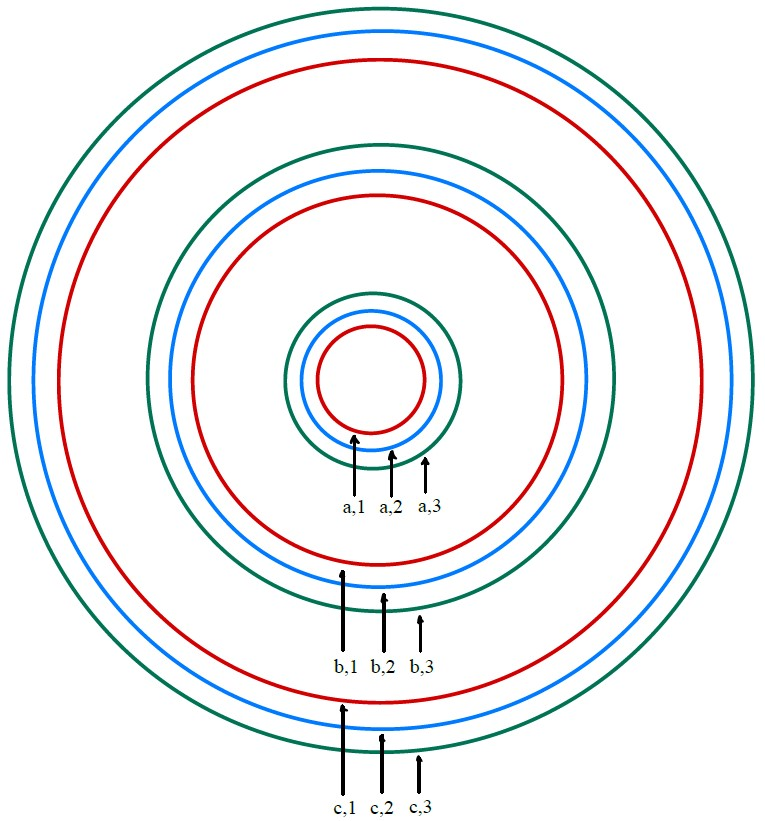
\includegraphics[scale=0.4]{scheme}
                \captionsetup{justification=centering, font=footnotesize}
                \captionof{figure}{Experimentální uspořádání aparatury.}
                \label{fig:scheme}
                \vspace{10pt}
                \raggedright   

            \subsection{Poissonovo rozdělení a $\chi^2$ test}
                Poissonovo rozdělení je pravděpodobnostní rozdělení diskrétní náhodné veličiny, která udává pravděpodobnost, že se daná událost stane $n$-krát v daném časovém intervalu nebo prostorovém objemu. Pravděpodobnostní funkce Poissonova rozdělení je dána vztahem (2):
                \begin{equation}
                    P(n) = \frac{\lambda^n}{n!} e^{-\lambda}
                \end{equation}
                kde $\lambda$ je střední hodnota a rozptyl Poissonova rozdělení.
                \par Pro ověření, zda počty zaznamenaných $\alpha$-částic mají Poissonovo rozdělení, můžeme použít $\chi^2$ test. Pro tento test je třeba spočítat hodnotu $\chi^2$ podle vztahu (3):
                \begin{equation}
                    \chi^2 = \sum_{j=1}^{n} \frac{(K_j(n) - NP_j(n))^2}{NP_j(n)}
                \end{equation}
                kde $K_j(n)$ je počet pozorovaných hodnot v určitém časovém intervalu, $P_j(n)$ je pravděpodobnost, že se daná událost stane $n$-krát v daném časovém intervalu a $N$ je celkový počet pozorování.
    \end{minipage}
\newpage
    \begin{minipage}[t]{0.5\textwidth} 
        \section{Měření}
            \subsection{Rutherfordův rozptyl}
                Abychom zjistili, zda rozložení detekovaných částic splňuje Rutherfordův rozptyl (2), měřili jsme počet $\alpha$-částic dopadajících na detektor $N$ v závislosti na vzdálenosti fólie od detektoru $f$ za čas $t$. Poté jsme vypočítali koeficient $x$ uvedený ve vzorci (2) a průměrný počet $\alpha$-částic dopadajících na detektor za 60 sekund $n$. Výsledky jsou uvedeny v tabulce (1).
                \par Vynesli jsme do grafu závislost $n(f)$, ze které je patrné, že rozložení počtu $\alpha$-částic dopadajících na detektor závisí na vzdálenosti fólie od detektoru. Výsledky jsou znázorněny na obrázku (2).
                \par Dále jsme nakreslili graf závislosti $n(x)$. Výsledky jsou znázorněny na obrázku (3). Lineárním fitováním jsme získali koeficient úměrnosti $K$: 
                \begin{center}
                    $K$ = (489 $\pm$ 78) [min$^{-1}$cm$^{-4}$]
                \end{center}
                
                Podle vzorce (2) jsme vypočítali teoretickou hodnotu $n$, přičemž vypočtenou hodnotu $x$ jsme dosadili do získané hodnoty koeficientu úměrnosti $K$. Výsledky jsou znázorněny v grafu (2). 

                \vspace{10pt}   
                \par \centering
                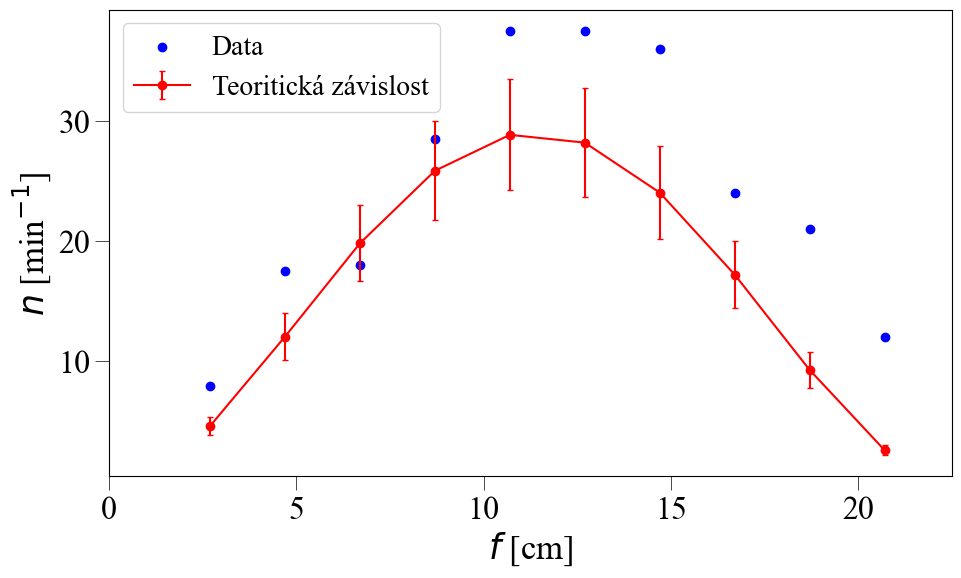
\includegraphics[scale=0.33]{n(f)}
                \captionsetup{justification=centering, font=footnotesize}
                \captionof{figure}{Závislost mnoství detekovaných $\alpha$-částic na vzdálenosti fólie od detektoru.}
                \label{fig:n(f)}
                \vspace{10pt}
                \raggedright   

                \vspace{10pt}   
                \par \centering
                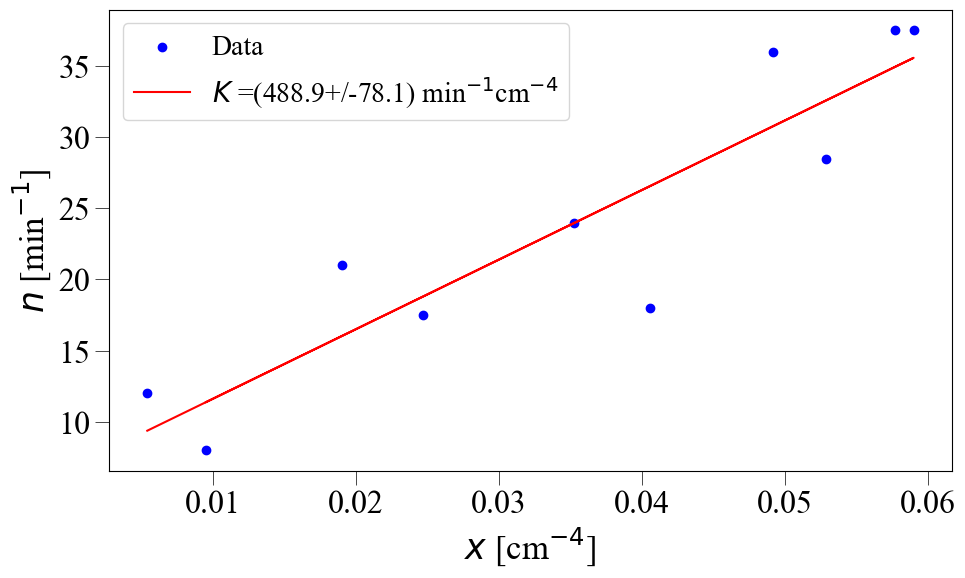
\includegraphics[scale=0.33]{n(x)}
                \captionsetup{justification=centering, font=footnotesize}
                \captionof{figure}{Závislost mnoství detekovaných $\alpha$-částic na x}
                \label{fig:n(x)}
                \vspace{10pt}
                \raggedright 
    \end{minipage}
    \hspace{10pt}
    \begin{minipage}[t]{0.5\textwidth} 
            \subsection{Poissonovo rozdělení}
                Abychom ověřili, zda je rozložení detekovaných $\alpha$-částic Poissonovo, umístili jsme fólii doprostřed mezi zdroj částic a detektor $f$ = 11.35 cm. Po dobu $T$ = 2000 s jsme pomocí osciloskopu nepřetržitě měřili počet $\alpha$-částic dopadajících na detektor. Pro filtraci získaných dat jsme nastavili práh rovný $U_{tresh}$ = 0.24 V. 
                Získaná data jsme rozdělili do časových intervalů $t_{diff}$ = 60 s a získali jsme tak počet měření $N$ = 32. Výpočtem průměrné hodnoty počtu detekovaných částic za 60 sekund jsme získali střední počet detekovaných částic $\lambda$:
                \begin{center}
                    $\lambda$ = 19.91 min$^{-1}$. 
                \end{center}
                Abychom potvrdili, že rozdělení má skutečně Poissonův tvar, sestrojili jsme histogram počtu detekovaných $\alpha$-částic za 60 sekund $n$ a provedli fitování rozdělení pomocí knihovny scipy.stats.poisson. Výsledky jsou uvedeny na obrázku (4).

                \vspace{10pt}   
                \par \centering
                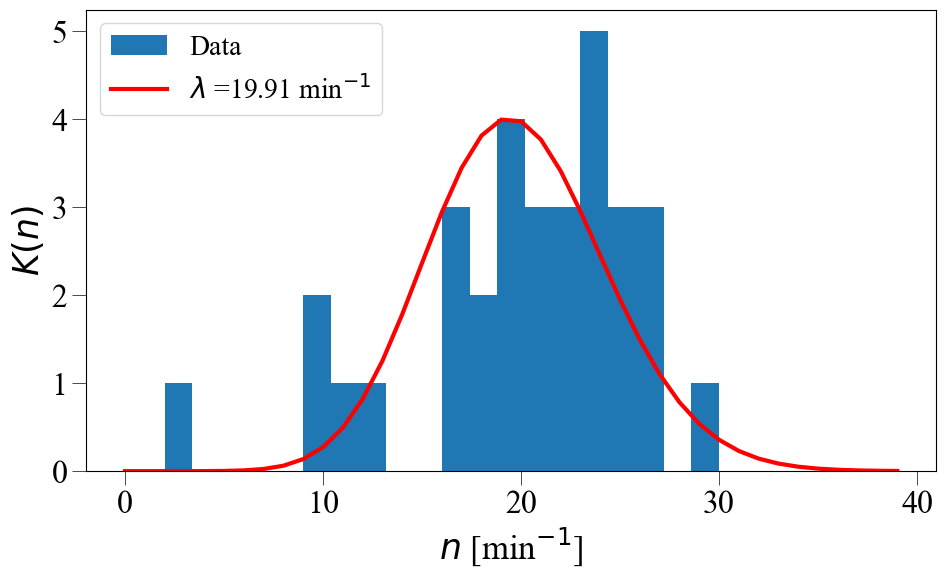
\includegraphics[scale=0.33]{K(n)}
                \captionsetup{justification=centering, font=footnotesize}
                \captionof{figure}{Histogram počtu detekovaných $\alpha$-částic za 60 sekund.}
                \label{fig:K(n)}
                \vspace{10pt}
                \raggedright 

                \par Abychom nakonec potvrdili hypotézu o povaze Poissonova rozdělení, použijeme test $\chi^2$. Rozdělme náš histogram na 5 nerovnoměrných intervalů $n$ tak, aby v každém z nich byla hodnota $K(n)$ > 5. Máme-li střední hodnotu Poissonova rozdělení $\lambda$ a počet měření $N$, použijeme vzorec (3) k nalezení hodnot NP(n) pro každý z intervalů $n$. Výsledky jsou uvedeny v tabulce (2). K výpočtu hodnoty $\chi^2$ použijte vzorec (4):
                \begin{center}
                    $\chi^2$ = 4.84
                \end{center}
                \vspace{10pt}
                \par K výpočtu veličin a jejich nejistot byla použita knihovna Uncertinties pro Python \cite{uncertainties}. Chyby byly rozšířeny o Studentův koeficient (2-Tail Confidence Level) s ohledem na stupně volnosti pro každou hodnotu, pro interval spolehlivosti 68.27\%.
    \end{minipage}
\newpage
        \section{Závěr} 
                \par Bylo zjištěno, že rozložení detekovaných $\alpha$-částic závisí na vzdálenosti fólie od detektoru. Bylo zjištěno, že rozložení detekovaných $\alpha$-částic splňuje Rutherfordův rozptyl. Byl získán koeficient úměrnosti $K$ = (489 $\pm$ 78) [min$^{-1}$cm$^{-4}$]. Z grafu (2) je patrné, že křivky naměřených a teoreticky vypočtených hodnot $n$ jsou v mezích chyby v intervalu 2.7 [cm]<$f$<8.7 [cm]. Pak mají hodnoty přibližně stejný posun ($n_{teor}$<$n_{naměř}$). Tvar křivek je v tomto případě podobný. Rozdíly mezi hodnotami $n_{teor}$ a $n_{naměř}$ při $f$>8.7 [cm] mohou být způsobeny nepřesností měření počtu $\alpha$-částic dopadajících na detektor. 
                \vspace{10pt}
                \par Dále bylo zjištěno, že rozložení detekovaných $\alpha$-částic má Poissonovo rozdělení. Byla získána hodnota $\chi^2$ = 4.84, zatímco pro počet stupňů volnosti $dof$ = $N$ - 1 = 4 a hladinu spolehlivosti 95 \% je kritická hodnota $\chi^2_{krit}$ = 9.483. Protože námi získaná hodnota $\chi^2$ < $\chi^2_{krit}$, nemůžeme zamítnout teorii, že naše rozdělení je Poissonovo.

                \renewcommand{\refname}{Odkazy}
                \begin{thebibliography}{9}
                    \bibitem{uncertainties}
                        Uncertainties, Dostupné online: \url{https://pypi.org/project/uncertainties}
                \end{thebibliography} 

    \begin{center}
        \section{Appendix}
            \subsection{Tabulka naměřených hodnot pro Rutherfordův rozptyl}
                \pgfplotstabletypeset[
                col sep=comma, % Defines the separator, comma for CSV
                string type, % Treats columns as strings (not math mode)
                every head row/.style={before row=\toprule,after row=\midrule},
                every last row/.style={after row=\bottomrule},
                columns/f/.style={column name=f [cm]},
                columns/t/.style={column name=t [s]},
                columns/r_1/.style={column name=$r_1$ [cm]},
                columns/r_2/.style={column name=$r_2$ [cm]},
                columns/alpha/.style={column name=\alpha [^\circ]},
                columns/beta/.style={column name=\beta [^\circ]},
                columns/chi/.style={column name=\chi [^\circ]},
                columns/x/.style={column name=x [cm$^{-4}$]},
                columns/n/.style={column name=n [min$^{-1}$]},
                columns/n_teor/.style={column name=$n_{teor}$ [min$^{-1}$]},
                ]{data/chi2_out.csv}
    \end{center}
    \begin{center}
        \subsection{Tabulka naměřených hodnot pro ověření Poissonova rozdělení}
            \pgfplotstabletypeset[
                col sep=comma, % Defines the separator, comma for CSV
                string type, % Treats columns as strings (not math mode)
                every head row/.style={before row=\toprule,after row=\midrule},
                every last row/.style={after row=\bottomrule},
                columns/K/.style={column name=K_j(n)},
                columns/NP/.style={column name=NP_j(n)},
                ]{data/poiss_out.csv}
    \end{center}
\end{document}